\chapter{Bilan personnel du projet}
\section{Les compétences technique}
L’intégration d’une équipe performante, possédant de solides connaissances et compétences, m’a permis de me perfectionner dans la maitrise du Framework Django

J’ai notamment pu en apprendre davantage sur l’architecture des API, avec lesquelles je n’avais que très peu travaillé lors de mon projet l’année précédente. 

Le fait de travailler avec cette architecture m’a également permis d’utiliser et de parfaire les connaissances en base de données que j’ai pu acquérir au cours de ma formation. 

En effet, la création des vues permettant les communications entre le client et le serveur, m’a offert la possibilité de regarder de plus près le Framework Django, le Framework Django REST Framework ainsi que le Framework VueJs. 

Au cours de ce projet, j’ai pu faire face à des problématiques d’intégrations de nouvelles technologies dans une architecture préexistante ; MCA s’étant construit bien avant mon arrivée à Clarisys Informatique.

Au cours de cette année, il a aussi fallu que j’apprenne à travailler avec un nouvel environnement, à savoir Docker. C’était la première fois que j’avais l’opportunité de travailler sur un environnement entièrement conteneurisé.

De manière générale, j’ai pu au cours de cette année en apprendre beaucoup sur MCA et son fonctionnement, notamment au sujet des processus de mise à jour. Même s’il s’agit d’un logiciel extrêmement vaste et parfois complexe, je me sens chaque jour plus à l’aise avec son architecture ainsi qu’avec les termes métiers qui lui sont associés.

Ce projet m’a globalement appris à améliorer mes capacités de recherche lorsque je rencontrais un problème et qu’il fallait parcourir la documentation existante par exemple, mais également lorsqu’il fallait chercher des éléments de réponse directement dans le code de MCA. J’ai également pu mettre en place, concrétiser, tester des solutions de résolution face à des problèmes et mobiliser les compétences acquises via ma formation ainsi que mon expérience d’alternant.

Le projet de cette année a donc été riche d’enseignements techniques et m’a offert la possibilité de monter en compétence et de gagner en autonomie dans le domaine du développement Web FullStack.

 J’ai pu explorer davantage les possibilités offertes par le Framework Django ainsi que le Framework Vuejs et le développement Frontend de manière générale. Enfin, j’ai pu utiliser et perfectionner mes connaissances en base de données et en apprendre plus sur le fonctionnement du logiciel sur lequel je travaille au quotidien.
 \begin{figure}[hp]
    \centering
    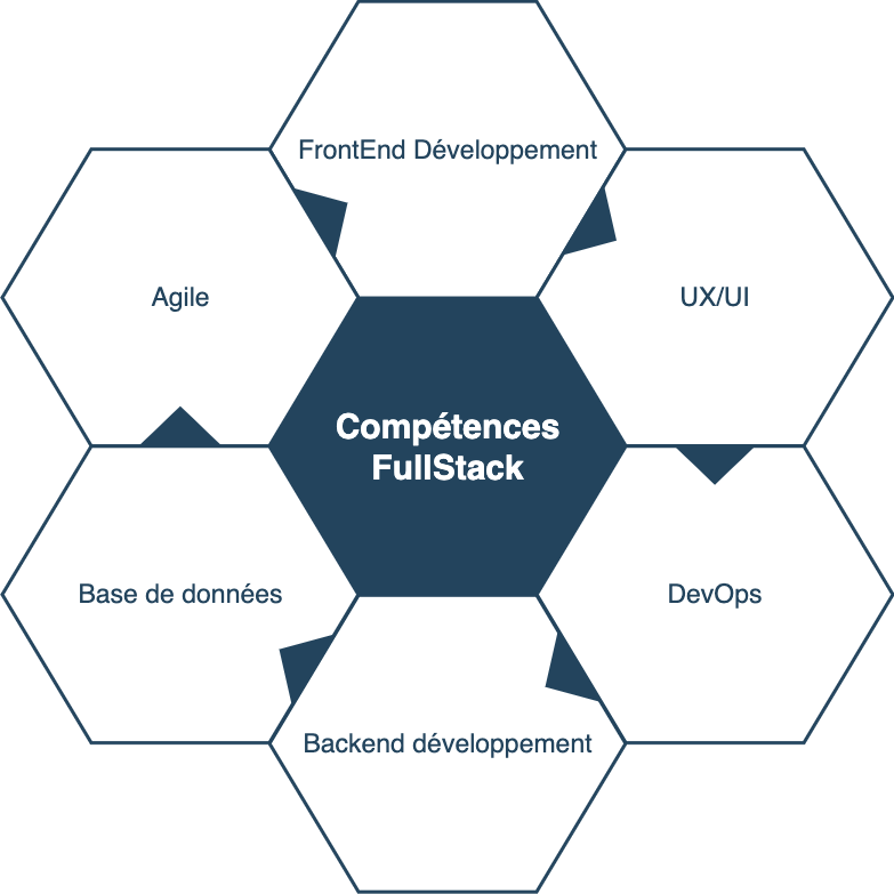
\includegraphics{images/skill_hard.png}
    \caption{Graphique de synthèse présentant les différentes compétences techniques acquises}
\end{figure}
\pagebreak

\section{Les compétences générales}
Au cours de ce projet, j’ai pu acquérir bien plus que des compétences techniques et informatiques. 

En effet, j’ai pu développer un grand nombre de compétences dites Soft Skills, indispensables pour tout futur ingénieur. 

Le fait de parcourir de nombreuses pages de documentation a non seulement amélioré mes capacités à rechercher une solution technique, mais cela m’a également permis de développer ma capacité à synthétiser et trier les informations à disposition.

Cette compétence informationnelle est pour moi essentielle lorsqu’on souhaite exercer le métier d’ingénieur puisqu’il s’agit d’une profession au sein de laquelle il est fréquent d’être confronté à l’inconnu.

En raison de l’alternance entre présentiel et télétravail, j’ai dû apprendre à m’adapter, à communiquer autrement avec mes collègues lorsqu’ils étaient en distanciel et je pense que cette adaptabilité va constituer une véritable force dans ma future carrière professionnelle.

Dans ce contexte particulier de crise sanitaire, j’ai également pu mieux mesurer les enjeux et besoins du domaine de la santé. 

En effet, si la crise du COVID-19 a pu impacter de manière négative de nombreuses entreprises, Clarisys Informatique, en raison de son statut d’éditeur de logiciel pour les laboratoires d’analyses médicales, a vu sa quantité de travail significativement augmenter. 

Plus que jamais, j’ai dû faire en sorte que mon travail soit conforme aux exigences et aux normes d’efficacité et de sécurité. 

A l’occasion du travail en distanciel, j’ai également pu acquérir une certaine autonomie au cours de ce projet. 

Même si mon maître d’apprentissage s’est rendu très disponible, j’ai également eu l’occasion de souvent travailler seul ce qui m’a permis d’apprendre à mieux m’organiser.

De plus, cela m’a aussi permis de mieux me connaître et de mettre en évidence mes qualités et mes défauts.

Enfin, j’ai bien sûr pu améliorer mes capacités relationnelles, en ayant des échanges réguliers avec mon maître d’apprentissage ainsi qu’avec l’ensemble de mes collègues. J’ai pu m’affirmer en présentant des réunions telles que le Daily Meeting ou encore les réunions de présentation du projet ayant lieu lors de l’amélioration continue. 

Lors de cette deuxième année d’alternance et la première au sein de Clarisys Informatique, j’ai donc pu améliorer mes compétences techniques mais également d’autres aspects clés plus formels et rationnels.
\pagebreak